
\documentclass[a4paper,12pt,oneside]{report}

\usepackage{colortbl}

\usepackage{phdthesis}

\usepackage{kostspielig}


\newcommand{\todo}[1]{\textcolor{red}{\textbf{TODO: #1}}}


\title{Questionnaires and Surveys}
\subtitle{Open-source web-app for questionnaires and surveys}
\date{Winter 2011}
\location{University of California Irvine}
\author{Kevin Brotcke\\
Maria Carrasco\\
Andrew Furusawa\\\
Joshua Papa }

\begin{document}
   
\renewcommand{\contentsname}{Contents}
\renewcommand{\bibname}{Bibliography}
\renewcommand{\caption}{{\bf Caption : }}

\raskolnikovmaketitle
\tableofcontents

\chapter{Introduction}
This document is the software requirements specification for an open source web application for questionnaires and surveys.

\section{Purpose}
This document outlines the online survey system describing its system requirements for the production of  a functional system, as well as user requirements in order to produce software compliant with the user's needs. We define the assumptions used to create the system, and provide use-case diagrams representing the system functionality and relationships.

The following  document is intended to be a third version of the requirements that must be formalized later. 

\subsection{Intended Audience and Reading Suggestions}
This document is intended for developers, project managers, users, testers and documentation writers. The main sections contained are an {\it Introduction} that contains information and instructions about the document. An {\it Overall Description} that gives a general idea of the product being specified in this SRS. The {\it Requirements}, describing the characteristics of the software. And the {\it Use Case Diagram}, to pressent a graphical overview of the functionality provided by the system.

\section{Definitions, acronyms, and abbreviations}
\begin{description}
\item[SRS] \emph{Software Requirements Specification.}
\item[DBMS] \emph{Data Base Management System}. The place where we will store the application data.
\item[CSS] \emph{Cascading Style Sheets}. Style sheet language used to describe the presentation semantics (the look and formatting) of a document.
\item[HTML] \emph{HyperText Markup Language}. Markup language for web pages.
\item[PHP] \emph{Hypertext Preprocessor}. Scripting language.
\item[DSL] \emph{Digital Subscriber Line}. Technology that provides digital data transmission over the wires of a local telephone network.
\item[FTP] \emph{File Transfer Protocol}. Standard network protocol used to copy a file from one host to another over a network.
\item[XLSX] \emph{File extension}. Excel Microsoft Office XML Format Spreadsheet.
\item[URL] \emph{Uniform Resource Locator} Specifies where an identified resource is available.
\end{description}

\section{References}
\begin{description}
\item [Project Webpage] {\it \url{  sites.google.com/site/inf117sprouse/home/}}
\item [IEEE Std 830-1998] {\it \url{ standards.ieee.org/findstds/standard/830-1998}}
\item [Repository] {\it \url{http://code.google.com/p/questionnaires-and-surveys/}}
\end{description}

\section{Overview}
Jon Sprouse of the Department of Cognitive Sciences at UCI is studying grammatical theory through surveys--both online and in the field. These surveys require careful construction through colors, ordering, and other various textual attributes to provide useful data for his work. In order to assist his research, a web-based system that generates these surveys provides efficiency and automation that would otherwise be done manually and intensively.


\chapter{Overall description}

\section{Product perspective}
This product aims to fill an existing need. Although there are many different choices for online survey generators, such as limeSurvey or SurveyMonkey, none of these options  seem to meet the requirements that are needed.

Developing into a web-based interface, the survey system is intended to contain customizable functionalities during survey creation, multiple version creation, and allow for survey participation. Customizations include both font attribute and layout manipulation, allowing the administrator to invoke different psychological responses from the participant. Multiple versions allow for the juxtaposition and analysis of participant responses with the use of "same-content, different-layout" environments.

\begin{figure}[h!]
  \begin{center}
   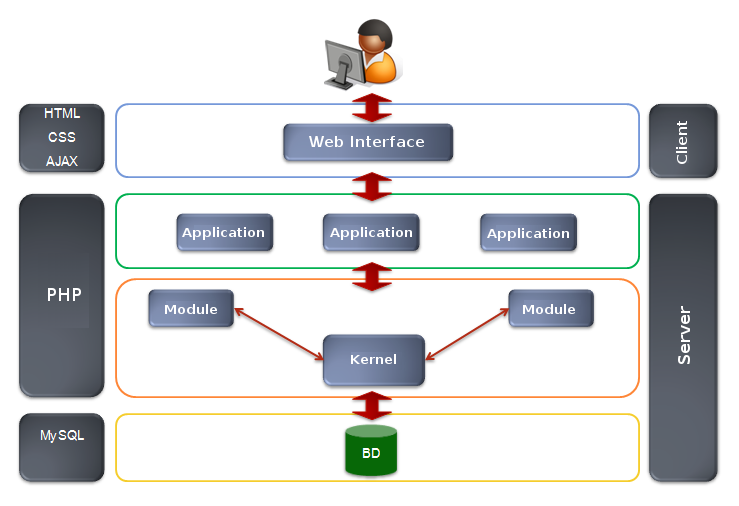
\includegraphics[width=14cm]{pics/ar.png}
  \end{center}
\caption{Block Diagram showing major components.}
\end{figure}

\subsection{System interfaces}
The software will have an {\it admin interface}. This interface will allow the administrator to perform several tasks.
\begin{itemize}
\item Upload experiments.
\item Download results.
\item Change appearance.
\begin{itemize}
\item Sample display at bottom that shows real time changes.
\end{itemize}
\end{itemize}

\subsection{User interfaces}
The main features that the software will present are:
\begin{itemize}
\item {\it Sets of surveys}, allowing the user to automatically loop through them.
\item {\it Pseudo-Randomization} of the order of the surveys.
\item {\it Result file}. This file will contain these main fields: Subject ID, survey number, code and responses.
\end{itemize}

\subsection{Hardware interfaces}
The software should run on a wide range of hardware. Please note that much of the computer equipment might have heterogeneous and unpredictable characteristics. Should the software run on a wide range of hardware. The web characteristics such as AJAX should not be abused because they do not work in older browsers and require more resources on the client side.

\subsection{Software interfaces}
The software should run on Windows. The software must be compatible with MS Excel and the main Internet web browsers such as Mozilla Firefox, Google Chrome and Internet Explorer.

\subsection{Communications interfaces}
The software must communicate with the clients' browsers via HTTP over TCP / IP.
\subsection{Memory}
There is no objective measure, but given the characteristics of the hardware described, it should be noted that the web portal should be light. There will not be more than two hundred surveys at the same time.


\subsection{Operations}
There are different roles in the organization that defines the operational mechanisms:
\begin{itemize}
\item The {\it Administrator} is responsible for uploading the surveys and questionnaires.
\item The {\it Participant} can register in the web page. It should be able to configure its preferences and consult its surveys and results.
\end{itemize}
\subsection{Site adaptation requirements}
There are no site adaptation requirements, besides those already discussed above.

\section{Product functions}
Broadly, the main functions of the software will be:
\begin{itemize}
\item Surveys management by the administrator.
\item Ability to answer the survey by the participants.
\end{itemize}
\section{User characteristics}
There are two different user types:
\begin{itemize}
	\item {\it Administator}. Middle class people with different computer literacy. Assumptions:
\begin{itemize}
	\item Has the ability to transfer files over FTP.
       	\item Must have an Admin account to login to manage surveys.
        \item The Administrator should be able to use the Control Panel to DL/UL surveys to/from the server.
        \item Ability to edit xlsx files and understand how to apply attributes to the survey prior to upload.
\end{itemize}
	\item {\it Participant}. Young people who are very familiar with the technologies. They will have to access to the URL for a given experiment.
\end{itemize}

%\section{Constraints}
\section{Assumptions and dependencies}

These requirements have been developed by making some assumptions based on characteristics of users and the general descriptions of equipment on which it will use the software. % These requirements may have additional costs deducted and the customer may consider deleting it finds that there has been an over-specification of the software.
 \chapter {Requirements}
\section{External interfaces}
\subsection{User interface}
\begin{itemize}
	\item Should be a web interface.
	\item Should follow the W3C standards.
	\item Should follow AA accessibility standards.
\end{itemize}
\subsection{Software interface}
\begin{itemize}
	\item Server installed with PHP 5.
	\item Internet connection with DSL or Cable bandwith.
	\item {\it xlsx} Microsoft Excel Version $\geq$ 07
	\item Latest version of Internet Explorer, Firefox, or Chrome as the Web browser.
\end{itemize}

\section{Functional Requirements}

\subsection {Survey}
\begin{itemize}
	\item A set of surveys consist of an experiment.
	\item For a given experiment, all surveys must be evenly distributed randomly to the user
       	\begin{itemize}   
		\item The user picks the experiment but is automatically assigned a survey
               	\item The user does not know which survey they are taking
	\end{itemize}
        \item Must support pseudo randomization
	\begin{itemize}
                \item The first letter of the survey code must not be next to another question with the same letter.
	\end{itemize}
       	\item Auto-complete must be disabled
\end{itemize}

\subsubsection { Appearance Of Surveys}

\begin{itemize} 
	\item  the appearance of the sentences on the web form (font, size, color, spacing, location, etc) needs to be customizable through CSS/HTML tags
	\item The web form needs to accept a couple of different response types (radio buttons, text boxes, etc)
	\item Left/Center/Right justifiable
	\item Autocomplete off
	\item \emph{CSS} template file option
	\item Sentences per page
\end{itemize}
\subsubsection{Administrator}
The administrator shall be able to do the following actions:
\begin{itemize}
	\item Create Survey \\ transfer a new xlsx file via ftp to an input folder
	\item Edit Survey \\ overrides the existing xlsx file
	\item View Survey \\ downloads the xlsx file from the server
	\item Download Results 
\end{itemize}

\subsubsection{Participant}
The participant shall be able to perform the following actions:
\begin{itemize}
	\item Request Survey by URL \\ Correct survey automatically assigned to user based off URL.
	\item Submit Survey Response
\end{itemize}

\subsection{ Input}
\begin{itemize} 
	\item Uses {\it xlsx} format as input file.
	\item  Input is read from a file containing:
	\begin{itemize}
        	\item Code - A unique identifier used for analysis. Only the Administrator sees this.
         	\item Question - The actual question the user must answer.
          	\item Format - Can be either Radio Button or Text Box. A survey may consist of all of one type or a combination of the two.
	\end{itemize}
   	\item Options in input file:
	\begin{itemize}
        	\item  Justification
         	\item Pagination
         	\item CSS file
         	\item Header Title
         	\item Table HTML Properties
         	\item Number of spaces between types of questions
	\end{itemize}
\end{itemize}

\subsection{Output}
\begin{itemize}
        \item The system shall have an option to export survey results. 
	\item The fields that shall be present in the file are:
	\begin{itemize}
		\item subject ID 
		\item survey number 
		\item code 
		\item responses
	\end{itemize}
\end{itemize}

\section{Performance requirements}
\begin{itemize}
	\item Surveys will be generated within 2 seconds.
\end{itemize}
\section{Logical database requirements}
The information stored in the database will be regarding to the experiments and surveys. 
%This should specify the logical requirements for any information that is to be placed into a database. This
%may include the following:
%a) Types of information used by various functions;
%b) Frequency of use;
%c) Accessing capabilities;
%d) Data entities and their relationships;
%e) Integrity constraints;
%f) Data retention requirements.
\section{Software system attributes}
\subsection{Ease of use}
\begin{itemize}
	\item Installation and maintenance for the Administrator must be very easy.
\end{itemize}


\subsection{Availability}
The software should have no interruptions in service except the following conditions: 
\begin{itemize}
	\item updating some of the service dependencies: DBMS, HTTP server, Web Server or operating system. 
	\item system re-installation. 
	\item Update from older versions of software.
\end{itemize}

\subsection{Portability}    
\begin{itemize}
	\item The pages generated must be 100$\%$ compatible
	\item To ensure compatibility with other browsers, XHTML 1.0 standard should be used for generated pages.
\end{itemize}




\chapter{Use Cases}

\section{Introduction}
Specified below are the different use cases of the application, that allows to study the interaction between user and system to achieve the functionality specified above.

\begin{figure}[h]
  \begin{center}
   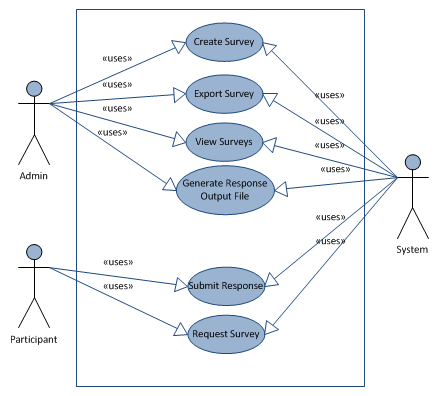
\includegraphics[width=13.3cm]{pics/usecase.png}
  \end{center}
 \caption{Use Case Diagram}
\end{figure}

\section{Use case list}
\begin{description}
\item [\ref{create}] Create Survey.
\item [\ref{manage}] Manage Surveys
\begin{description}
\item [\ref{edit}]  Edit Survey.
\item [\ref{view}] View Surveys.
\item [\ref{output}] Generate response output file.
\end{description}
\item [\ref{submit}]Submit response.
\item [\ref{request}]Request Survey.

\end{description}

\section{Use Cases}


\subsection{Create survey}
\label{create}


\begin{figure}[h!]
  \begin{center}
   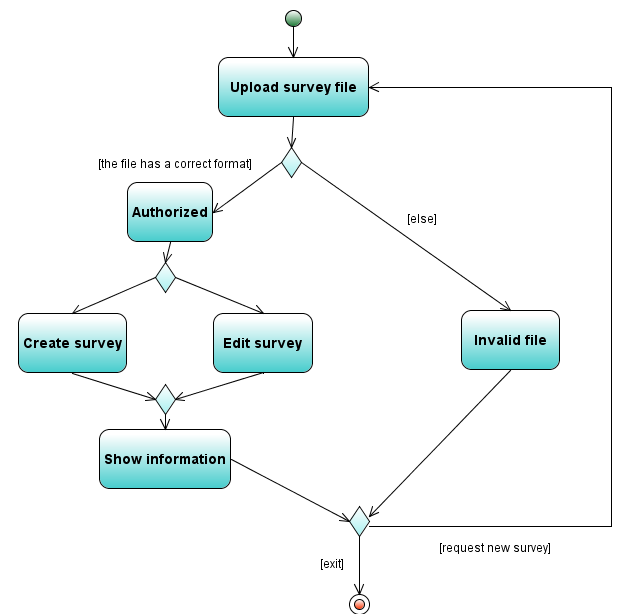
\includegraphics[width=14.6cm]{pics/Activity.png}
  \end{center}
 \caption{Activity Diagram}
\end{figure}


\setlength{\extrarowheight}{1.5mm}
\begin{tabular}{|>{\columncolor[rgb]{.3,.4,.9}}p{3.1cm} |>{\columncolor{white}} p{10.4cm} |}  \hline\hline
  \textcolor{white}{{\bf Name}} & Create Survey\\ \hline
  \textcolor{white}{{\bf Description}} & The administrator of the application creates an experiment.\\ \hline
  \textcolor{white}{{\bf Dependencies }} & None. \\ \hline
  \textcolor{white}{{\bf Actors}} & Administrator \\ \hline
  \textcolor{white}{{\bf Preconditions}} & User should have access to the system. \\  \hline
  \textcolor{white}{{\bf Postconditions}} & A new survey will be created.\\  \hline\hline
\end{tabular}


\begin{tabular}[]{|p{13.8cm}|}\hline
  \rowcolor[rgb]{.3,.4,.9}\textcolor{white}{{\bf Basic Path}} \\\hline
\end{tabular}

\begin{tabular}[]{|p{6.7cm}|p{6.7cm}|}\hline
  \rowcolor[gray]{0.9} User & System \\\hline
  1.- Access to the option Create Survey, through the main menu. & 2.- Shows an option to upload survey files. \\\hline
  3.- Select the file to upload and press OK. & 4.- Checks the validity of data. \\\hline
  & 5.- Confirms the creation of the survey.\\\hline
\end{tabular}\\ 

\begin{tabular}[]{|p{13.8cm}|}\hline
  \rowcolor[rgb]{.3,.4,.9}\textcolor{white}{{\bf Alternative Paths }} \\\hline
\end{tabular}\\ 

\begin{tabular}[]{|p{6.7cm}|p{6.7cm}|}\hline
  \rowcolor[gray]{0.9} User & System \\\hline
  & 5b.- The data is incorrect. Asks for another file input. \\\hline
\end{tabular}

\begin{figure}[h!]
  \begin{center}
   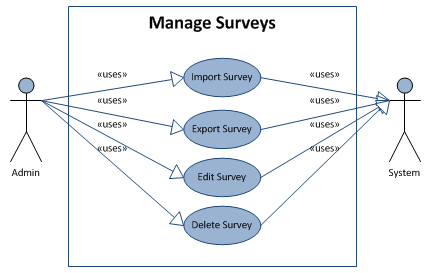
\includegraphics[width=13.6cm]{pics/ManageSurveys.png}
  \end{center}
 \caption{Use Case Diagram}
\end{figure}

\subsection{Manage Surveys}
\label{manage}

\begin{figure}[h!]
  \begin{center}
   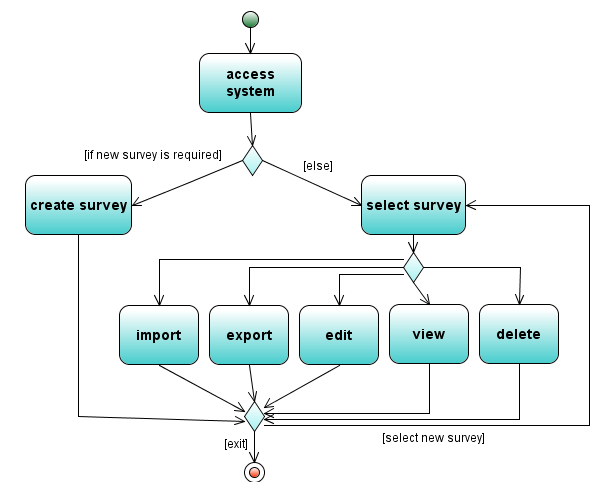
\includegraphics[width=13.3cm]{pics/Activity2.png}
  \end{center}
 \caption{Activity Diagram}
\end{figure}
\subsubsection{ Edit survey}
\label{edit}

\setlength{\extrarowheight}{1.5mm}
\begin{tabular}{|>{\columncolor[rgb]{.3,.4,.9}}p{3.1cm} |>{\columncolor{white}} p{10.4cm} |}  \hline\hline
  \textcolor{white}{{\bf Name}} & Edit Survey\\ \hline
  \textcolor{white}{{\bf Description}} & The user edits an existing survey. \\ \hline
  \textcolor{white}{{\bf Dependencies }} & \ref{create}  \\ \hline
  \textcolor{white}{{\bf Actors}} & Administrator \\ \hline
  \textcolor{white}{{\bf Preconditions}} & A survey must have been already created. \\ \hline
  \textcolor{white}{{\bf Postconditions}} & An existing survey will be changed.\\ \hline\hline
\end{tabular}


\begin{tabular}{|p{13.8cm}|}\hline
  \rowcolor[rgb]{.3,.4,.9}\textcolor{white}{{\bf Basic Path}} \\\hline
\end{tabular}

\begin{tabular}[]{|p{6.7cm}|p{6.7cm}|}\hline
  \rowcolor[gray]{0.9} User & System \\\hline
  1.- Choose the option {\it Edit survey} in the menu. & 2.- Shows the options for editing the file. \\\hline
  3.- Chage the options and  press OK. & 4.- Checks validity of data. \\\hline
  & 5.- Confirms the edition of the survey.\\\hline
\end{tabular}\\ 

\begin{tabular}[]{|p{13.8cm}|}\hline
  \rowcolor[rgb]{.3,.4,.9}\textcolor{white}{{\bf Alternative Paths }} \\\hline
\end{tabular}\\ 

\begin{tabular}[]{|p{6.7cm}|p{6.7cm}|}\hline
  \rowcolor[gray]{0.9} User & System \\\hline
  & 5b.- The data is incorrect. Returns to step 2.\\\hline
\end{tabular}

\subsubsection{ View Surveys}
\label{view}

\setlength{\extrarowheight}{1.5mm}
\begin{tabular}{|>{\columncolor[rgb]{.3,.4,.9}}p{3.1cm} |>{\columncolor{white}} p{10.4cm} |}  \hline\hline
  \textcolor{white}{{\bf Name}} & View Surveys\\ \hline
  \textcolor{white}{{\bf Description}} & The user views the existing surveys.\\ \hline
  \textcolor{white}{{\bf Dependencies }} & \ref{create}  \\ \hline
  \textcolor{white}{{\bf Actors}} & Administrator \\ \hline
  \textcolor{white}{{\bf Preconditions}} & The user must have access to the system. \\\hline
  \textcolor{white}{{\bf Postconditions}} & The survey(s) will be displayed on the screen.\\\hline\hline
\end{tabular}


\begin{tabular}{|p{13.8cm}|}\hline
  \rowcolor[rgb]{.3,.4,.9}\textcolor{white}{{\bf Basic Path}} \\\hline
\end{tabular}

\begin{tabular}[]{|p{6.7cm}|p{6.7cm}|}\hline
  \rowcolor[gray]{0.9} User & System \\\hline
  1.- Choose the option {\it View surveys}. & 2.- Displays a menu, with all the current surveys in the system. \\\hline
  3.- Choose a survey within the given list. & 4.- Shows the selected survey. \\\hline
\end{tabular}\\ 

\begin{tabular}[]{|p{13.8cm}|}\hline
  \rowcolor[rgb]{.3,.4,.9}\textcolor{white}{{\bf Alternative Paths }} \\\hline
\end{tabular}\\ 

\begin{tabular}[]{|p{6.7cm}|p{6.7cm}|}\hline
  \rowcolor[gray]{0.9} User & System \\\hline
  & 2b.- There are no surveys in the system. Displays the message: {\it There are no surveys available.} \\\hline
  & 4b.- If the systems fails while accessing the required data, it returns to step 2.   \\\hline
\end{tabular}

\subsection{ Generate Response Output File}
\label{output}

\setlength{\extrarowheight}{1.5mm}
\begin{tabular}{|>{\columncolor[rgb]{.3,.4,.9}}p{3.1cm} |>{\columncolor{white}} p{10.4cm} |}  \hline\hline
  \textcolor{white}{{\bf Name}} & Generate response output file.\\ \hline
  \textcolor{white}{{\bf Description}} & Generates an output file containing all surveys responses. \\\hline
  \textcolor{white}{{\bf Dependencies }} & \ref{create}  \ref{submit}\\ \hline
  \textcolor{white}{{\bf Actors}} & Administrator \\ \hline
  \textcolor{white}{{\bf Preconditions}} & A survey must have been already created and submited. \\ \hline
  \textcolor{white}{{\bf Postconditions}} & An output file will be created.\\ \hline\hline
\end{tabular}


\begin{tabular}{|p{13.8cm}|}\hline
  \rowcolor[rgb]{.3,.4,.9}\textcolor{white}{{\bf Basic Path}} \\\hline
\end{tabular}

\begin{tabular}[]{|p{6.7cm}|p{6.7cm}|}\hline
  \rowcolor[gray]{0.9} User & System \\\hline
  1.- Choose the option {\it Generate Response File}. & 2.- Shows a list with all the current surveys. \\\hline
  3.- Selects a survey from which to obtain the output file and selects Ok. & 4.- Displays a window with Saving options. \\\hline
  5.- Selects a path where to store the output file, and a name for the file. Clicks {\it Save} & 6.- Performs the operation and displays an operation completed message.\\\hline
\end{tabular}\\ 

\begin{tabular}[]{|p{13.8cm}|}\hline
  \rowcolor[rgb]{.3,.4,.9}\textcolor{white}{{\bf Alternative Paths }} \\\hline
\end{tabular}\\ 

\begin{tabular}[]{|p{6.7cm}|p{6.7cm}|}\hline
  \rowcolor[gray]{0.9} User & System \\\hline
  & 6b.- The operation could not be done. No file was generated. Returns to step 2. \\\hline
\end{tabular}

\subsection{Request Survey }
\label{request}

\begin{figure}[h!]
  \begin{center}
   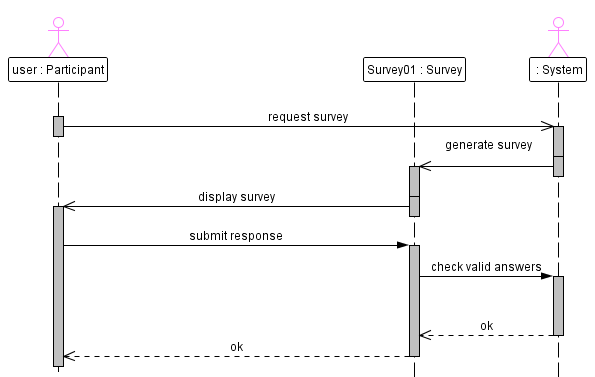
\includegraphics[width=15cm]{pics/Sequence.png}
  \end{center}
 \caption{Sequence Diagram}
\end{figure}

\setlength{\extrarowheight}{1.5mm}
\begin{tabular}{|>{\columncolor[rgb]{.3,.4,.9}}p{3.1cm} |>{\columncolor{white}} p{10.4cm} |}  \hline\hline
  \textcolor{white}{{\bf Name}} & Request Survey\\\hline
  \textcolor{white}{{\bf Description}} & The user request a new survey to be displayed. \\\hline
  \textcolor{white}{{\bf Dependencies }} & \ref{create}  \\\hline
  \textcolor{white}{{\bf Actors}} & Participant \\ \hline
  \textcolor{white}{{\bf Preconditions}} & A survey must have been already created. \\ \hline
  \textcolor{white}{{\bf Postconditions}} & A survey will be displayed.\\ \hline\hline
\end{tabular}


\begin{tabular}{|p{13.8cm}|}\hline
  \rowcolor[rgb]{.3,.4,.9}\textcolor{white}{{\bf Basic Path}} \\\hline
\end{tabular}

\begin{tabular}[]{|p{6.7cm}|p{6.7cm}|}\hline
  \rowcolor[gray]{0.9} User & System \\\hline
  1.- Enters the URL in the web browser. & 2.- Shows the main menu to the user. \\\hline
  3.- Selects the option {\it Request Survey}. & 4.- Presents a list of surveys . \\\hline
  4.- Chooses a survey. & 6.- Displays a version of the selected survey.\\\hline
\end{tabular}\\ 

\begin{tabular}[]{|p{13.8cm}|}\hline
  \rowcolor[rgb]{.3,.4,.9}\textcolor{white}{{\bf Alternative Paths }} \\\hline
\end{tabular}\\ 

\begin{tabular}[]{|p{6.7cm}|p{6.7cm}|}\hline
  \rowcolor[gray]{0.9} User & System \\\hline
  &  \\\hline
\end{tabular}

\subsection{ Submit Response}
\label{submit}

\setlength{\extrarowheight}{1.5mm}
\begin{tabular}{|>{\columncolor[rgb]{.3,.4,.9}}p{3.1cm} |>{\columncolor{white}} p{10.4cm} |}  \hline\hline
  \textcolor{white}{{\bf Name}} & Submit Response\\ \hline
  \textcolor{white}{{\bf Description}} & The user submits a fully completed survey. \\\hline
  \textcolor{white}{{\bf Dependencies }} & \ref{request}  \\\hline
  \textcolor{white}{{\bf Actors}} & Participant \\\hline
  \textcolor{white}{{\bf Preconditions}} & A survey must have been already requested. \\\hline
  \textcolor{white}{{\bf Postconditions}} & A survey response will be submitted.\\\hline\hline
\end{tabular}


\begin{tabular}{|p{13.8cm}|}\hline
  \rowcolor[rgb]{.3,.4,.9}\textcolor{white}{{\bf Basic Path}} \\\hline
\end{tabular}

\begin{tabular}[]{|p{6.7cm}|p{6.7cm}|}\hline
  \rowcolor[gray]{0.9} User & System \\\hline
  1.- Choose the option {\it Submit Survey}. & 2.- Stores the data and Shows a congratulations message. \\\hline
\end{tabular}\\ 

\begin{tabular}[]{|p{13.8cm}|}\hline
  \rowcolor[rgb]{.3,.4,.9}\textcolor{white}{{\bf Alternative Paths }} \\\hline
\end{tabular}\\ 

\begin{tabular}[]{|p{6.7cm}|p{6.7cm}|}\hline
  \rowcolor[gray]{0.9} User & System \\\hline
  &  2b.- If there are any incomplete box, shows the survey again.  \\\hline
\end{tabular}


\chapter{Analysis}
\section{Class Diagram}


\begin{figure}[h]
  \begin{center}
  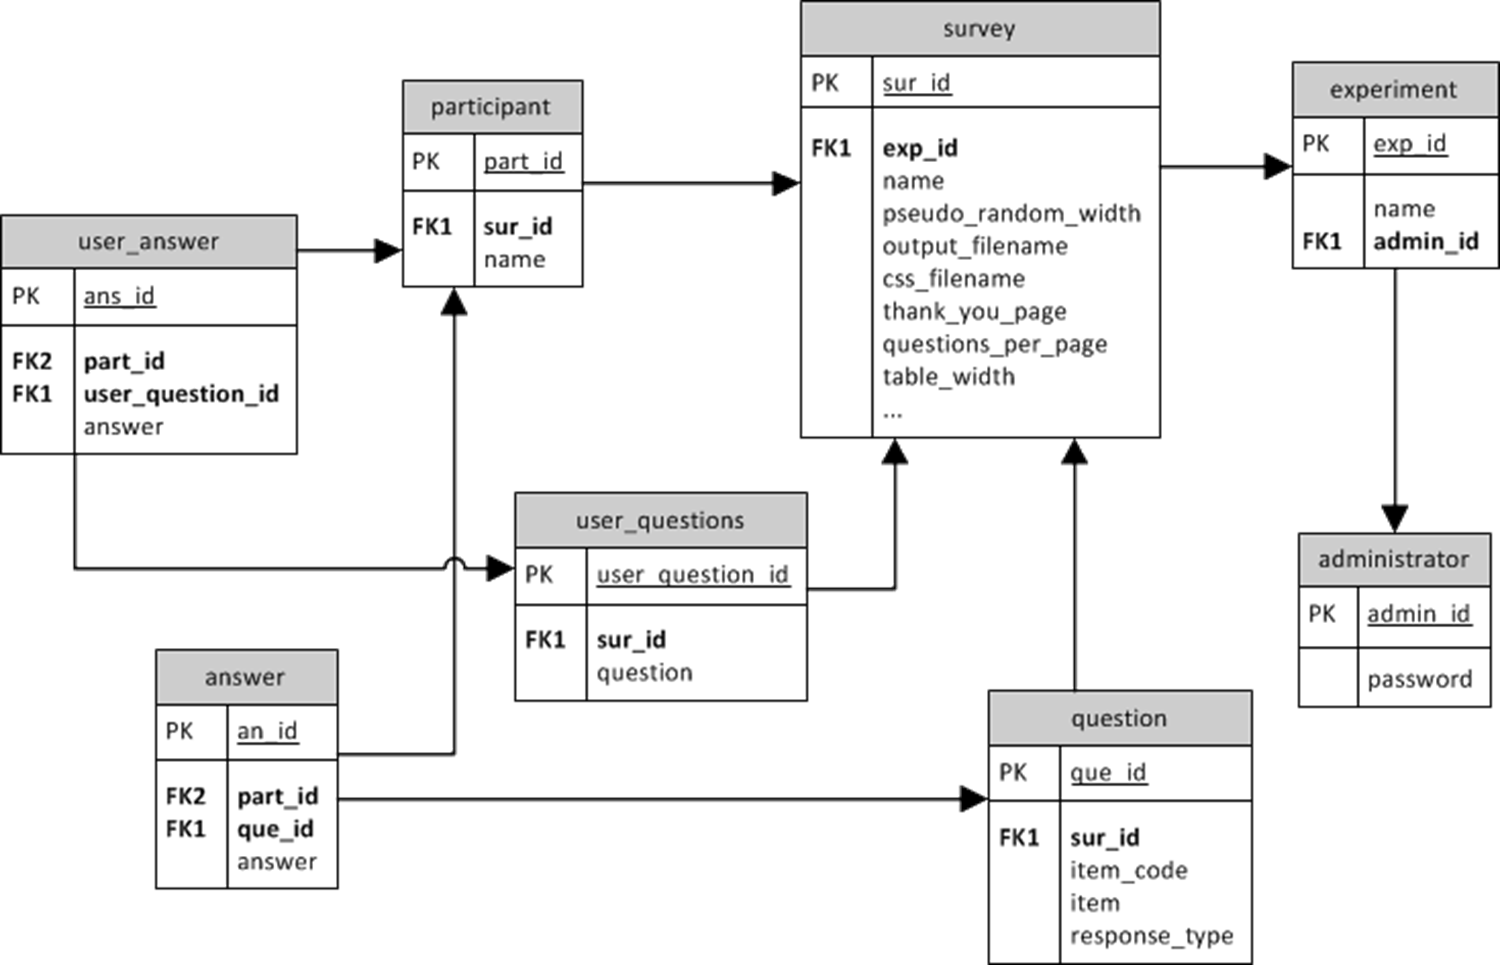
\includegraphics[width=16.2cm]{pics/class.png}
  \end{center}
 \caption{Class Diagram}
\end{figure}


\pagebreak
\begin{thebibliography}{XXX}
\bibitem{1} Stevens, P. \& Pooley, R., 1999. {\it USING UML. Software Engineering with objects and components}. $2^{nd}$ed. Harlow Essex: Addison Wesley \\
\bibitem{2} Britton, C. \& Doake, J., 2005. {\it A student guide to OBJECT-ORIENTED DEVELOPMENT }.Burlington, MA: Elsevier Butterworth-Heinemann\\
\end{thebibliography}


\end{document}
